% titulo: Capítulo IV – Análisis y presentación de resultados
% estado: borrador
% actualizado: 2026-11-18
% Corte del 18-nov-2026 (registro S-19 de Tesis-Doc/README.md). Las cifras salen de
% agente/evaluacion/resultados/resumen.json y se regeneran con `python -m tools.eval_dataset todo --tesis`.
% Solo cubre las reglas con evaluador a la fecha (RE-20 y RE-21). Al cierre del Sprint 6 se actualiza con las reglas
% de citas y referencias y con las sugerencias de Gemini.

\chapter{Análisis y Presentación de Resultados}\label{cap:resultados}

Este capítulo presenta la evaluación del agente al 18 de noviembre de 2026. A esa fecha el agente tiene dos reglas con evaluador: RE-20, que exige un tamaño mínimo de 531 $\times$ 1328 píxeles por figura, y RE-21, que exige una resolución de al menos 300 puntos por pulgada (dpi). Los resultados son de esas dos reglas. Las reglas de citas y referencias y las sugerencias redactadas con Gemini se incorporan al cierre del Sprint 6.

\section{Datos de la evaluación}\label{sec:dataset}

La evaluación usa un \emph{dataset} sintético (Sección~\ref{sec:evaluacion}). Sus manuscritos no vienen de autores reales. Los produce un generador que decide, a partir de una semilla, qué defectos lleva cada documento y los anota en un manifiesto. Ese manifiesto es la verdad de referencia contra la que se compara el agente.

El generador se diseñó para que la verdad de referencia no dependa del agente. Se tomaron cuatro medidas.

\begin{itemize}
  \item Los manuscritos se escriben con las plantillas oficiales de la revista. Una parte se compila con pdfLaTeX y la otra se exporta a PDF con Microsoft Word, que son los dos caminos que siguen los autores.
  \item El generador no usa el código del agente ni su librería de lectura de PDF (PyMuPDF).
  \item La página de cada figura la informan LaTeX y Word, no el agente.
  \item Las imágenes guardadas en cada PDF se leen con una segunda librería (pypdf) para confirmar que el PDF contiene lo que el manifiesto dice.
\end{itemize}

Los textos de los manuscritos son ficticios y los redactó Gemini a partir de una instrucción fija: 33 artículos de cinco áreas de la computación, sin autores, instituciones ni referencias reales. Gemini solo aporta la redacción y no decide ningún defecto. No se usó ningún manuscrito real, de modo que no hay datos personales.

Cada documento recibe uno de tres perfiles: conforme, con un defecto o con varios defectos. Cada figura recibe un tamaño en píxeles y una resolución tomados de listas que incluyen valores claramente correctos, claramente incorrectos y valores en el borde de cada umbral, como 530, 531 y 532 píxeles de alto o 299, 300 y 301 dpi. Además, cada figura tiene una variante que describe cómo la insertó el autor. La Tabla~\ref{tab:4-1} las resume.

{\small
\begin{longtable}{@{}>{\raggedright\arraybackslash}p{0.150\textwidth}>{\raggedright\arraybackslash}p{0.530\textwidth}>{\raggedright\arraybackslash}p{0.120\textwidth}>{\raggedright\arraybackslash}p{0.100\textwidth}@{}}
\caption{Variantes de figura del \emph{dataset} sintético}\label{tab:4-1}\\
\toprule
\textbf{Variante} & \textbf{Descripción} & \textbf{Generador} & \textbf{Figuras} \\
\midrule
\endfirsthead
\toprule
\textbf{Variante} & \textbf{Descripción} & \textbf{Generador} & \textbf{Figuras} \\
\midrule
\endhead
\bottomrule
\endfoot
\endlastfoot
\texttt{png} & Imagen PNG insertada tal cual & LaTeX y Word & 308 \\
\texttt{jpeg} & Imagen JPEG insertada tal cual & LaTeX y Word & 85 \\
\texttt{png\_alfa} & Imagen PNG con canal de transparencia & LaTeX y Word & 38 \\
\texttt{recortada} & La imagen guardada es más ancha que la parte que se ve, porque el autor la recortó dentro del documento & LaTeX & 32 \\
\texttt{rotada} & La imagen está guardada de lado y el documento la gira 90 grados & LaTeX & 33 \\
\texttt{vectorial} & Gráfico dibujado con líneas y formas, sin píxeles; las dos reglas no le aplican & LaTeX & 27 \\
\textbf{Total} &  &  & \textbf{523} \\
\end{longtable}
}

La unidad de análisis es la decisión, es decir, un par formado por una figura y una regla. Para cada decisión hay cuatro resultados posibles: verdadero positivo ($VP$) si la figura incumple la regla y el agente lo reporta, falso positivo ($FP$) si el agente reporta un incumplimiento que no existe, falso negativo ($FN$) si el incumplimiento existe y el agente no lo reporta, y verdadero negativo ($VN$) si la figura cumple y el agente no reporta nada.

El agente se ejecutó como una caja negra. Cada PDF se envió por \texttt{POST /manuscripts} y los hallazgos se leyeron de \texttt{GET /manuscripts/\{id\}/findings}. Cada documento se envió tres veces y se tomó la mediana del tiempo.

\section{Análisis e interpretación de datos}

\subsection{Uso de estadística descriptiva}

\subsubsection*{Composición del \emph{dataset}}

El \emph{dataset} tiene 200 documentos y 523 figuras. La Tabla~\ref{tab:4-2} muestra su composición. Los 200 documentos se analizaron completos y terminaron en estado \texttt{validated}; ninguno quedó como ilegible o fallido. El agente reportó al menos un hallazgo en 163 de ellos.

{\small
\begin{longtable}{@{}>{\raggedright\arraybackslash}p{0.330\textwidth}>{\raggedright\arraybackslash}p{0.570\textwidth}@{}}
\caption{Composición del \emph{dataset} sintético (semilla 20261118)}\label{tab:4-2}\\
\toprule
\textbf{Característica} & \textbf{Valor} \\
\midrule
\endfirsthead
\toprule
\textbf{Característica} & \textbf{Valor} \\
\midrule
\endhead
\bottomrule
\endfoot
\endlastfoot
Documentos & 200: 140 compilados con LaTeX y 60 exportados con Word \\
Perfil & 46 conformes, 108 con un defecto y 46 con varios \\
Tipo de artículo & 50 cortos, 104 originales y 46 de revisión \\
Páginas por documento & Media 8,5; mediana 8; desviación estándar 3,0; mínimo 4; máximo 16 \\
Figuras por documento & Media 2,6; mediana 3; mínimo 0; máximo 5. Hay 8 documentos sin figuras \\
Figuras & 523: 496 de píxeles y 27 vectoriales \\
Decisiones evaluadas & 992: 496 por cada regla \\
Incumplimientos reales en el PDF & 238 de RE-20 y 260 de RE-21 \\
\end{longtable}
}

\subsubsection*{Resultados por regla}

La Tabla~\ref{tab:4-3} presenta la matriz de confusión de cada regla y las métricas que se calculan con ella. Además de la precisión, el \emph{recall} y $F_1$, definidos en la Sección~\ref{sec:evaluacion}, se informa la especificidad, que es la proporción de figuras conformes que el agente deja sin observar: $VN / (VN + FP)$.

{\small
\begin{longtable}{@{}>{\raggedright\arraybackslash}p{0.100\textwidth}>{\raggedleft\arraybackslash}p{0.060\textwidth}>{\raggedleft\arraybackslash}p{0.060\textwidth}>{\raggedleft\arraybackslash}p{0.060\textwidth}>{\raggedleft\arraybackslash}p{0.060\textwidth}>{\raggedleft\arraybackslash}p{0.110\textwidth}>{\raggedleft\arraybackslash}p{0.090\textwidth}>{\raggedleft\arraybackslash}p{0.070\textwidth}>{\raggedleft\arraybackslash}p{0.140\textwidth}@{}}
\caption{Matriz de confusión y métricas por regla}\label{tab:4-3}\\
\toprule
\textbf{Regla} & \textbf{VP} & \textbf{FP} & \textbf{FN} & \textbf{VN} & \textbf{Precisión} & \textbf{Recall} & \textbf{F1} & \textbf{Especificidad} \\
\midrule
\endfirsthead
\toprule
\textbf{Regla} & \textbf{VP} & \textbf{FP} & \textbf{FN} & \textbf{VN} & \textbf{Precisión} & \textbf{Recall} & \textbf{F1} & \textbf{Especificidad} \\
\midrule
\endhead
\bottomrule
\endfoot
\endlastfoot
RE-20 & 231 & 23 & 7 & 235 & 0,909 & 0,971 & 0,939 & 0,911 \\
RE-21 & 259 & 16 & 1 & 220 & 0,942 & 0,996 & 0,968 & 0,932 \\
\textbf{Ambas} & \textbf{490} & \textbf{39} & \textbf{8} & \textbf{455} & \textbf{0,926} & \textbf{0,984} & \textbf{0,954} & \textbf{0,921} \\
\end{longtable}
}

El agente acertó en 945 de las 992 decisiones (95,3 \%). De los 47 errores, 39 son falsos positivos y 8 son falsos negativos. El agente, entonces, se equivoca más por observar figuras que están bien que por dejar pasar figuras que están mal.

\subsubsection*{Resultados por generador y por variante}

La Tabla~\ref{tab:4-4} separa los resultados según el programa que produjo el PDF. Los 39 falsos positivos están en documentos de LaTeX. En ese subconjunto la precisión baja a 0,795 en RE-20 y a 0,861 en RE-21.

{\small
\begin{longtable}{@{}>{\raggedright\arraybackslash}p{0.100\textwidth}>{\raggedright\arraybackslash}p{0.120\textwidth}>{\raggedleft\arraybackslash}p{0.070\textwidth}>{\raggedleft\arraybackslash}p{0.070\textwidth}>{\raggedleft\arraybackslash}p{0.070\textwidth}>{\raggedleft\arraybackslash}p{0.070\textwidth}>{\raggedleft\arraybackslash}p{0.120\textwidth}>{\raggedleft\arraybackslash}p{0.100\textwidth}@{}}
\caption{Resultados por regla y generador del PDF}\label{tab:4-4}\\
\toprule
\textbf{Regla} & \textbf{Generador} & \textbf{VP} & \textbf{FP} & \textbf{FN} & \textbf{VN} & \textbf{Precisión} & \textbf{Recall} \\
\midrule
\endfirsthead
\toprule
\textbf{Regla} & \textbf{Generador} & \textbf{VP} & \textbf{FP} & \textbf{FN} & \textbf{VN} & \textbf{Precisión} & \textbf{Recall} \\
\midrule
\endhead
\bottomrule
\endfoot
\endlastfoot
RE-20 & LaTeX & 89 & 23 & 6 & 217 & 0,795 & 0,937 \\
RE-20 & Word & 142 & 0 & 1 & 18 & 1,000 & 0,993 \\
RE-21 & LaTeX & 99 & 16 & 0 & 220 & 0,861 & 1,000 \\
RE-21 & Word & 160 & 0 & 1 & 0 & 1,000 & 0,994 \\
\end{longtable}
}

La Tabla~\ref{tab:4-5} y la Figura~\ref{fig:errores-variante} muestran dónde están los errores. Se concentran en dos variantes. Las figuras rotadas producen los 39 falsos positivos y las figuras recortadas producen 5 de los 8 falsos negativos. En las variantes \texttt{jpeg} y \texttt{png\_alfa} no hubo ningún error, y en las 27 figuras vectoriales el agente no emitió ningún hallazgo, que es lo correcto.

{\small
\begin{longtable}{@{}>{\raggedright\arraybackslash}p{0.160\textwidth}>{\raggedleft\arraybackslash}p{0.100\textwidth}>{\raggedleft\arraybackslash}p{0.130\textwidth}>{\raggedleft\arraybackslash}p{0.130\textwidth}>{\raggedleft\arraybackslash}p{0.130\textwidth}>{\raggedleft\arraybackslash}p{0.130\textwidth}@{}}
\caption{Errores por variante de figura}\label{tab:4-5}\\
\toprule
\textbf{Variante} & \textbf{Figuras} & \textbf{FP en RE-20} & \textbf{FN en RE-20} & \textbf{FP en RE-21} & \textbf{FN en RE-21} \\
\midrule
\endfirsthead
\toprule
\textbf{Variante} & \textbf{Figuras} & \textbf{FP en RE-20} & \textbf{FN en RE-20} & \textbf{FP en RE-21} & \textbf{FN en RE-21} \\
\midrule
\endhead
\bottomrule
\endfoot
\endlastfoot
\texttt{png} & 308 & 0 & 2 & 0 & 1 \\
\texttt{jpeg} & 85 & 0 & 0 & 0 & 0 \\
\texttt{png\_alfa} & 38 & 0 & 0 & 0 & 0 \\
\texttt{recortada} & 32 & 0 & 5 & 0 & 0 \\
\texttt{rotada} & 33 & 23 & 0 & 16 & 0 \\
\texttt{vectorial} & 27 & 0 & 0 & 0 & 0 \\
\textbf{Total} & \textbf{523} & \textbf{23} & \textbf{7} & \textbf{16} & \textbf{1} \\
\end{longtable}
}

\begin{figure}[H]
  \centering
  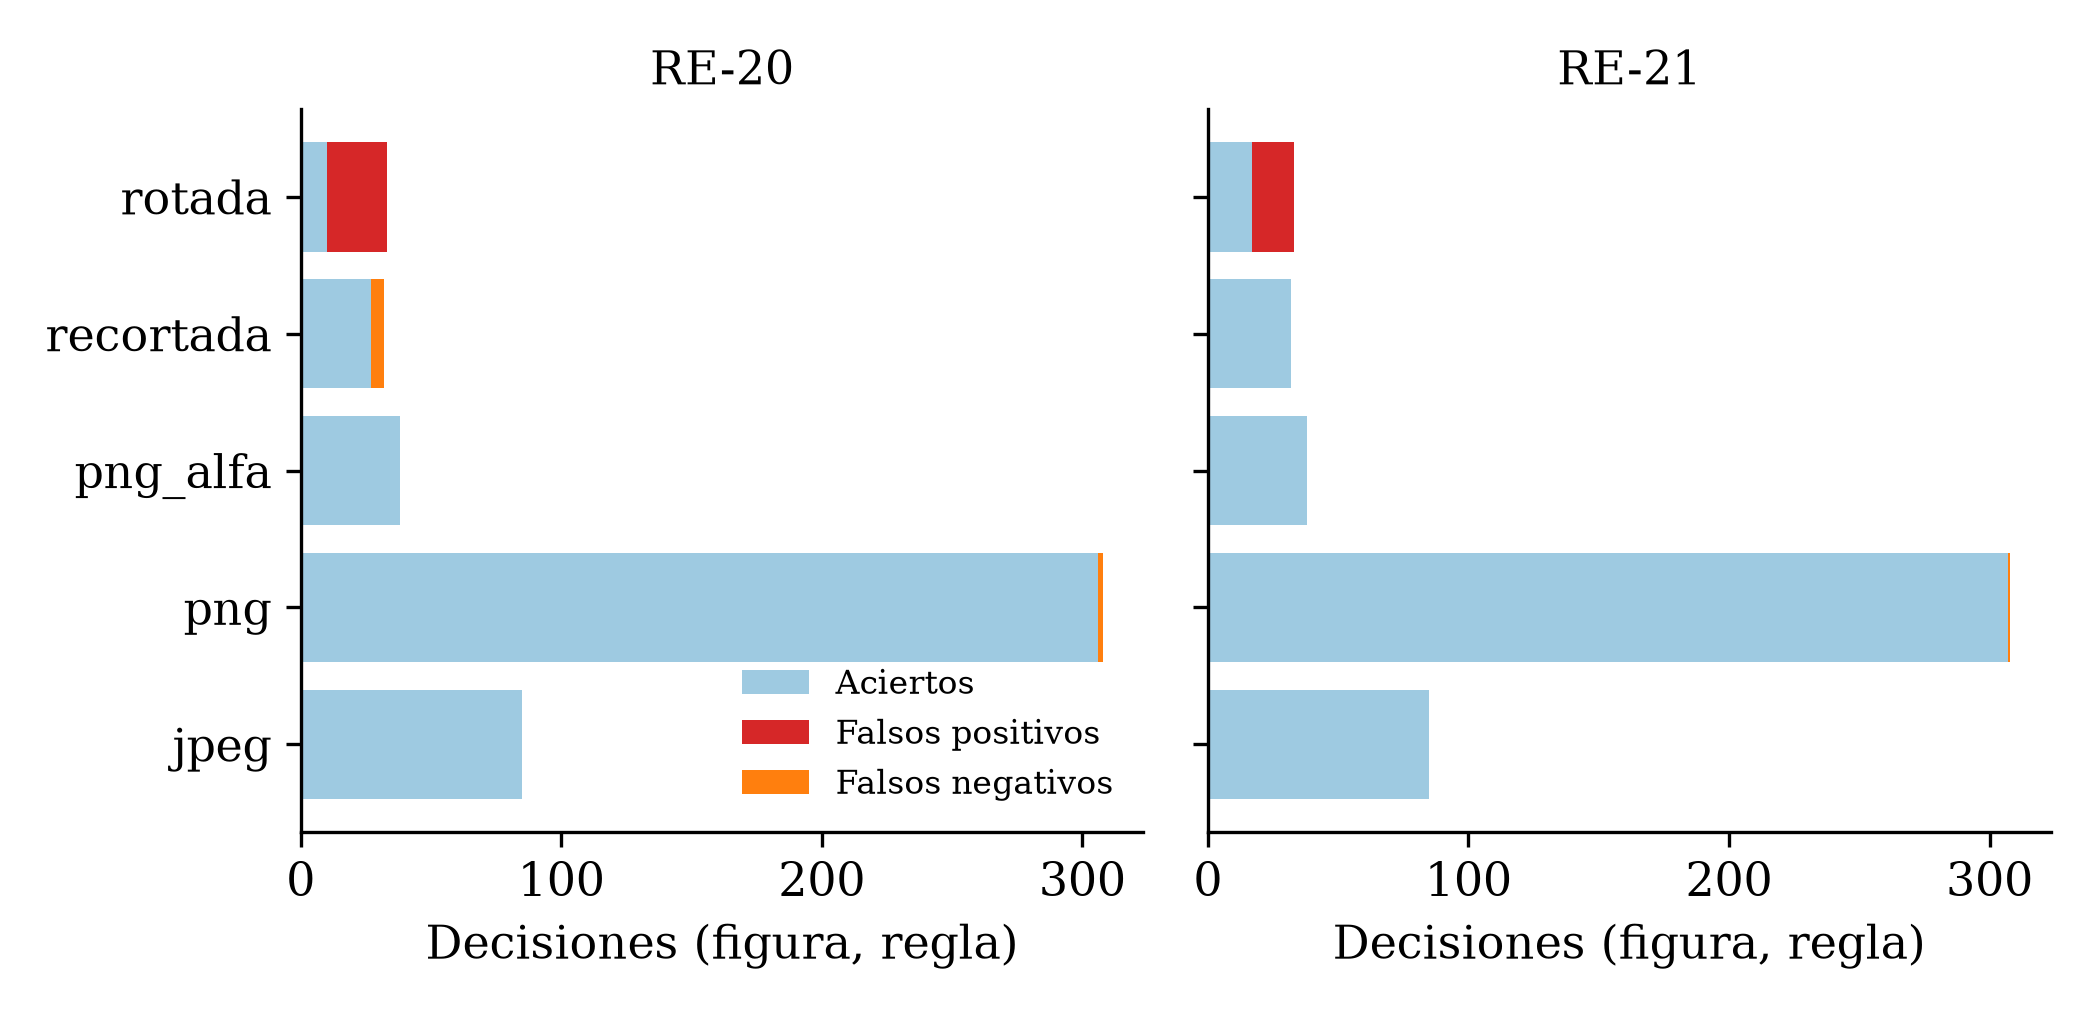
\includegraphics[width=\textwidth]{figuras/resultados/errores-por-variante.png}
  \caption{Aciertos y errores del agente por variante de figura y por regla}
  \label{fig:errores-variante}
\end{figure}

\subsubsection*{Efecto de la conversión a PDF}

La verificación independiente de los PDF mostró algo que no estaba previsto en el diseño. LaTeX guarda cada imagen en el PDF tal como el autor la insertó. Word no lo hace. Al exportar a PDF, Word redujo a unos 200 puntos por pulgada todas las imágenes que el autor había insertado a 280 dpi o más, aunque el documento tenía activada la opción de no comprimir imágenes. La Tabla~\ref{tab:4-6} muestra el efecto.

{\small
\begin{longtable}{@{}>{\raggedright\arraybackslash}p{0.520\textwidth}>{\raggedleft\arraybackslash}p{0.170\textwidth}>{\raggedleft\arraybackslash}p{0.170\textwidth}@{}}
\caption{Efecto de la conversión a PDF sobre las figuras de píxeles}\label{tab:4-6}\\
\toprule
\textbf{Indicador} & \textbf{LaTeX} & \textbf{Word} \\
\midrule
\endfirsthead
\toprule
\textbf{Indicador} & \textbf{LaTeX} & \textbf{Word} \\
\midrule
\endhead
\bottomrule
\endfoot
\endlastfoot
Figuras de píxeles & 335 & 161 \\
Figuras que el conversor redujo & 0 & 141 (88 \%) \\
Cumplen RE-21 en el documento de origen & 236 & 117 \\
\quad de ellas, incumplen RE-21 en el PDF & 0 & 117 (100 \%) \\
Cumplen RE-20 en el documento de origen & 240 & 117 \\
\quad de ellas, incumplen RE-20 en el PDF & 0 & 99 (85 \%) \\
\end{longtable}
}

Ninguna figura de un documento de Word llegó al PDF con 300 dpi. Como el agente recibe el PDF, la verdad de referencia se fijó sobre lo que el PDF contiene. Por eso las 117 figuras de la Tabla~\ref{tab:4-6} cuentan como incumplimientos reales y no como errores del agente.

\subsubsection*{Tiempo de análisis}

La Tabla~\ref{tab:4-7} resume el tiempo que tomó analizar cada documento, desde que la API recibe el PDF hasta que los hallazgos quedan guardados. La Figura~\ref{fig:tiempo-paginas} lo relaciona con el número de páginas.

{\small
\begin{longtable}{@{}>{\raggedright\arraybackslash}p{0.180\textwidth}>{\raggedleft\arraybackslash}p{0.080\textwidth}>{\raggedleft\arraybackslash}p{0.100\textwidth}>{\raggedleft\arraybackslash}p{0.100\textwidth}>{\raggedleft\arraybackslash}p{0.130\textwidth}>{\raggedleft\arraybackslash}p{0.110\textwidth}>{\raggedleft\arraybackslash}p{0.100\textwidth}@{}}
\caption{Tiempo de análisis por documento, en segundos}\label{tab:4-7}\\
\toprule
\textbf{Conjunto} & \textbf{n} & \textbf{Media} & \textbf{Mediana} & \textbf{Desv. est.} & \textbf{Percentil 95} & \textbf{Máximo} \\
\midrule
\endfirsthead
\toprule
\textbf{Conjunto} & \textbf{n} & \textbf{Media} & \textbf{Mediana} & \textbf{Desv. est.} & \textbf{Percentil 95} & \textbf{Máximo} \\
\midrule
\endhead
\bottomrule
\endfoot
\endlastfoot
LaTeX & 140 & 0,32 & 0,31 & 0,13 & 0,51 & 1,09 \\
Word & 60 & 0,22 & 0,22 & 0,05 & 0,30 & 0,42 \\
\textbf{Todos} & \textbf{200} & \textbf{0,29} & \textbf{0,27} & \textbf{0,12} & \textbf{0,50} & \textbf{1,09} \\
\end{longtable}
}

\begin{figure}[H]
  \centering
  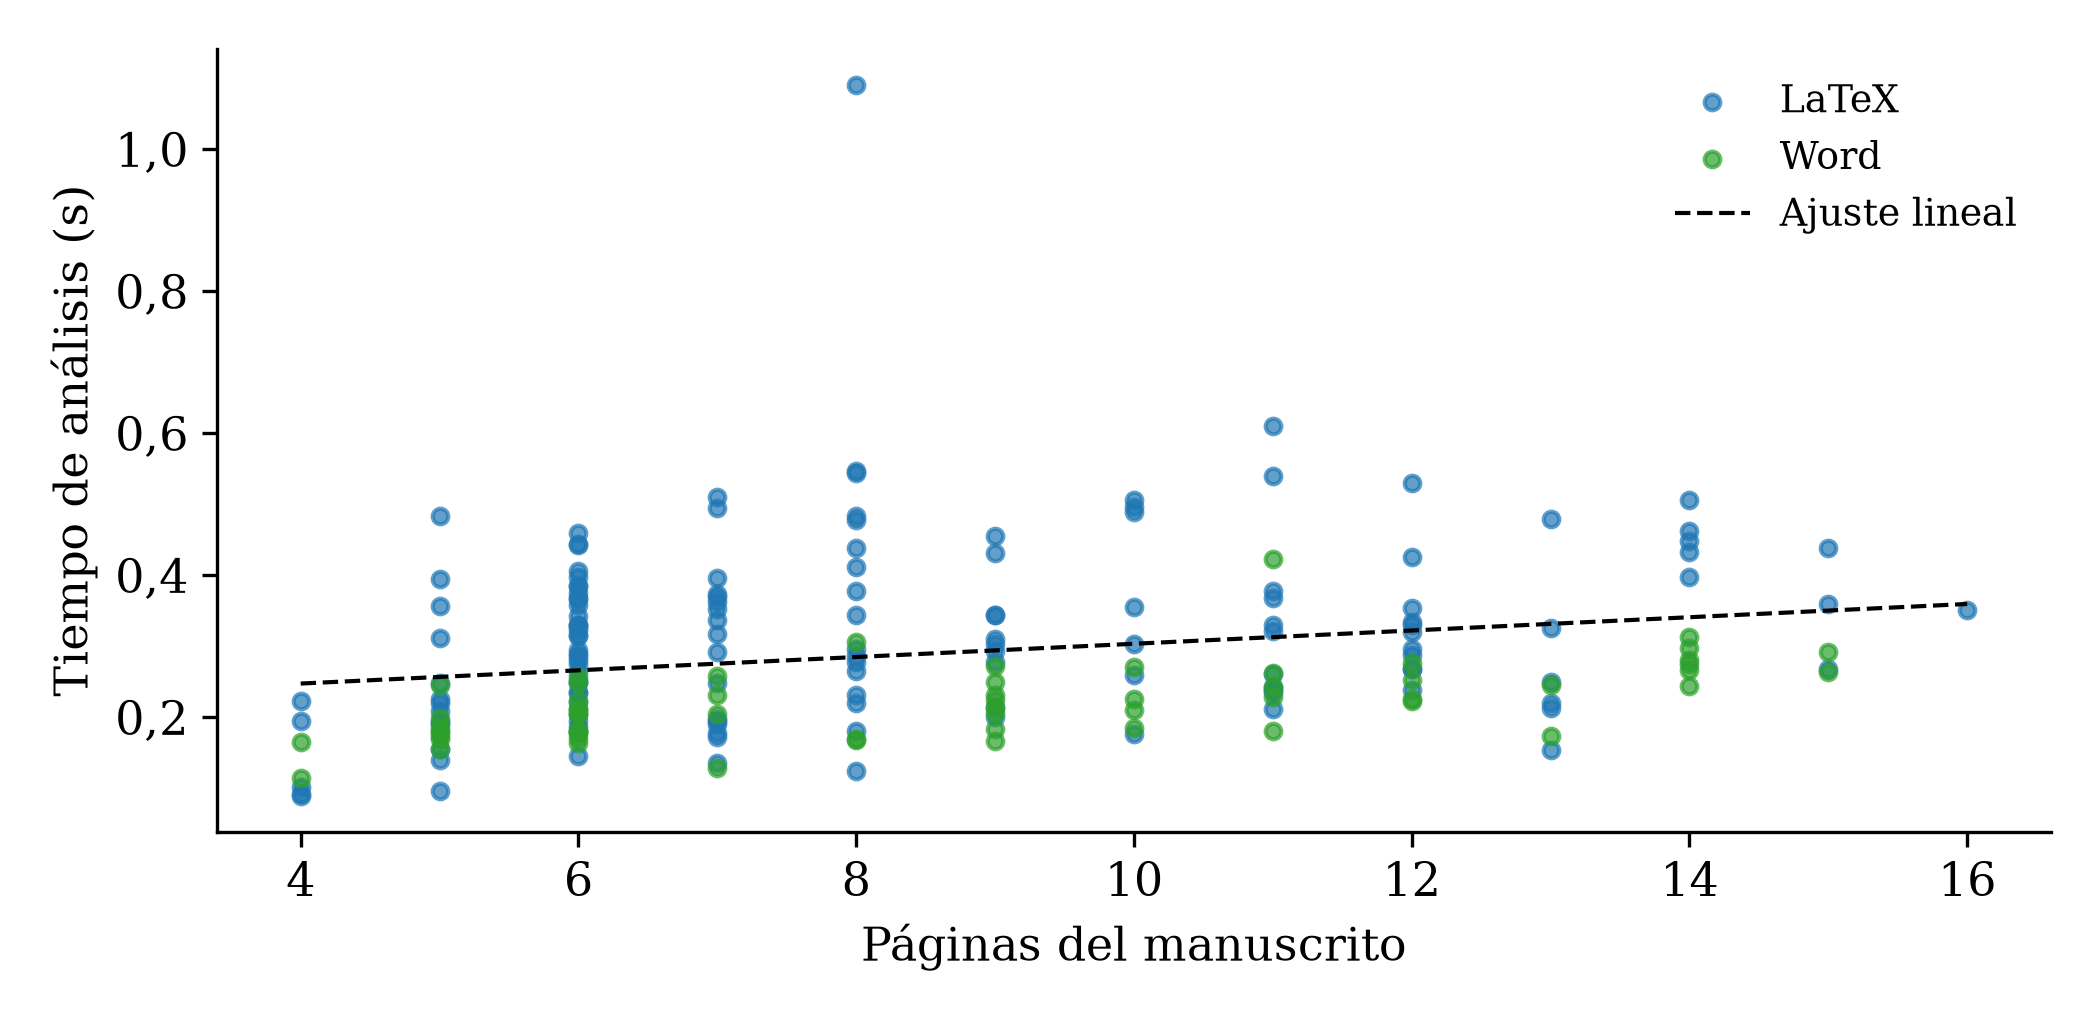
\includegraphics[width=\textwidth]{figuras/resultados/tiempo-por-paginas.png}
  \caption{Tiempo de análisis según el número de páginas del manuscrito}
  \label{fig:tiempo-paginas}
\end{figure}

El análisis más lento tomó 1,09 segundos. Los seis documentos de 15 páginas o más se analizaron en 0,44 segundos como máximo.

\subsection{Uso de estadística inferencial}

La estadística descriptiva dice qué pasó en estos 200 documentos. La inferencial responde otra pregunta: qué tan seguros se puede estar de que el agente se comportaría igual con otros documentos generados de la misma forma. Se usó un nivel de significancia de 0,05 en todas las pruebas.

\subsubsection*{Intervalos de confianza}

Para la precisión y el \emph{recall} se calculó el intervalo de confianza de Wilson al 95 \% \cite{ref37}. Se eligió este intervalo porque se comporta bien con proporciones cercanas a 1, que es el caso de estas métricas. La Tabla~\ref{tab:4-8} los presenta.

{\small
\begin{longtable}{@{}>{\raggedright\arraybackslash}p{0.180\textwidth}>{\raggedleft\arraybackslash}p{0.110\textwidth}>{\raggedright\arraybackslash}p{0.200\textwidth}>{\raggedleft\arraybackslash}p{0.090\textwidth}>{\raggedright\arraybackslash}p{0.200\textwidth}@{}}
\caption{Intervalos de confianza de Wilson al 95 \% para la precisión y el \emph{recall}}\label{tab:4-8}\\
\toprule
\textbf{Conjunto} & \textbf{Precisión} & \textbf{IC 95 \%} & \textbf{Recall} & \textbf{IC 95 \%} \\
\midrule
\endfirsthead
\toprule
\textbf{Conjunto} & \textbf{Precisión} & \textbf{IC 95 \%} & \textbf{Recall} & \textbf{IC 95 \%} \\
\midrule
\endhead
\bottomrule
\endfoot
\endlastfoot
RE-20, todos & 0,909 & [0,868; 0,939] & 0,971 & [0,941; 0,986] \\
RE-21, todos & 0,942 & [0,908; 0,964] & 0,996 & [0,979; 0,999] \\
RE-20, LaTeX & 0,795 & [0,711; 0,859] & 0,937 & [0,869; 0,971] \\
RE-21, LaTeX & 0,861 & [0,786; 0,913] & 1,000 & [0,963; 1,000] \\
RE-20, Word & 1,000 & [0,974; 1,000] & 0,993 & [0,962; 0,999] \\
RE-21, Word & 1,000 & [0,977; 1,000] & 0,994 & [0,966; 0,999] \\
\end{longtable}
}

\subsubsection*{Contraste con las metas}

Las metas del producto son una precisión de al menos 0,85 y un \emph{recall} de al menos 0,75 en las reglas determinísticas. Para saber si los valores observados superan esas metas más allá del azar, se aplicó una prueba binomial exacta de una cola a cada métrica. La hipótesis nula es que la proporción real es igual o menor que la meta, y la alternativa es que la supera. La Tabla~\ref{tab:4-9} muestra los resultados.

{\small
\begin{longtable}{@{}>{\raggedright\arraybackslash}p{0.180\textwidth}>{\raggedright\arraybackslash}p{0.150\textwidth}>{\raggedleft\arraybackslash}p{0.110\textwidth}>{\raggedleft\arraybackslash}p{0.080\textwidth}>{\raggedleft\arraybackslash}p{0.110\textwidth}>{\raggedright\arraybackslash}p{0.200\textwidth}@{}}
\caption{Prueba binomial exacta de cada métrica contra su meta}\label{tab:4-9}\\
\toprule
\textbf{Conjunto} & \textbf{Métrica} & \textbf{Observado} & \textbf{Meta} & \textbf{Valor p} & \textbf{Conclusión} \\
\midrule
\endfirsthead
\toprule
\textbf{Conjunto} & \textbf{Métrica} & \textbf{Observado} & \textbf{Meta} & \textbf{Valor p} & \textbf{Conclusión} \\
\midrule
\endhead
\bottomrule
\endfoot
\endlastfoot
RE-20, todos & Precisión & 0,909 & 0,85 & 0,003 & Supera la meta \\
RE-21, todos & Precisión & 0,942 & 0,85 & < 0,001 & Supera la meta \\
RE-20, todos & Recall & 0,971 & 0,75 & < 0,001 & Supera la meta \\
RE-21, todos & Recall & 0,996 & 0,75 & < 0,001 & Supera la meta \\
RE-20, LaTeX & Precisión & 0,795 & 0,85 & 0,957 & No se demuestra \\
RE-21, LaTeX & Precisión & 0,861 & 0,85 & 0,434 & No se demuestra \\
\end{longtable}
}

Con todos los documentos, las cuatro métricas superan su meta de forma significativa. En el subconjunto de LaTeX el resultado es distinto: la precisión de RE-20 queda por debajo de la meta y la de RE-21 la supera por tan poco que no se puede descartar el azar.

\subsubsection*{Diferencia entre generadores}

Para saber si el agente se equivoca más con un generador que con otro, se comparó la proporción de decisiones erradas con la prueba exacta de Fisher \cite{ref38}. En RE-20 el agente erró 29 de 335 decisiones en LaTeX y 1 de 161 en Word ($p < 0{,}001$). En RE-21 erró 16 de 335 en LaTeX y 1 de 161 en Word ($p = 0{,}016$). La diferencia es significativa en las dos reglas. Se explica por el diseño: las figuras rotadas y recortadas, que concentran los errores, solo existen en los documentos de LaTeX.

\subsubsection*{Relación entre el tiempo y el tamaño del documento}

Se calculó la correlación de Spearman \cite{ref39} entre el tiempo de análisis y dos medidas del tamaño del documento. Se eligió esta correlación porque no supone que los tiempos sigan una distribución normal. El tiempo crece con el número de páginas ($\rho = 0{,}31$; $p < 0{,}001$) y crece más con el número de figuras ($\rho = 0{,}47$; $p < 0{,}001$). Un ajuste lineal estima 0,009 segundos por página adicional ($R^2 = 0{,}06$) y 0,053 segundos por figura adicional ($R^2 = 0{,}22$). El tamaño del documento explica poco de la variación del tiempo, que en todos los casos es de fracciones de segundo.

\section{Estrategias para la presentación de resultados}

\subsection{Síntesis narrativa}

Se generaron 200 manuscritos sintéticos con 523 figuras y se le pidió al agente que los revisara. El agente analizó todos sin fallar y tomó 992 decisiones sobre dos reglas de figuras. Acertó en 945.

Cuando una figura incumple una regla, el agente casi siempre lo detecta: dejó pasar 8 de 498 incumplimientos. Cuando el agente reporta un incumplimiento, acierta en 490 de 529 casos. Los 39 reportes equivocados corresponden a una sola situación, la de las figuras guardadas de lado y giradas dentro del documento.

El análisis de un manuscrito toma menos de medio segundo en el 95 \% de los casos. La etapa de extracción y reglas, entonces, no es la que limita el tiempo total del agente.

El hallazgo más útil para la revista no es sobre el agente. Los manuscritos que se escriben en Word pierden resolución al convertirse a PDF. Un autor que inserta sus figuras a 300 dpi, como piden las directrices, entrega un PDF con figuras a unos 200 dpi.

\subsection{Síntesis cualitativa}

Se revisó cada uno de los 47 errores para identificar su causa. Todos se explican por tres causas, y las tres están en la extracción de figuras (US-06), no en los evaluadores de las reglas.

\begin{enumerate}
  \item \textbf{Figuras rotadas (39 falsos positivos).} El agente toma el ancho y el alto de la imagen tal como está guardada en el PDF y no considera el giro que el documento le aplica. Una figura que se ve de 1800 píxeles de ancho por 900 de alto se lee como de 900 de ancho por 1800 de alto, y se reporta como demasiado angosta. La resolución también se calcula mal, porque se divide el ancho guardado entre el ancho impreso, que corresponde al otro lado de la imagen: esa misma figura, insertada a 300 dpi, se reportó con 150 dpi.
  \item \textbf{Figuras recortadas (5 falsos negativos).} Cuando el autor recorta una imagen dentro del documento, el PDF conserva la imagen completa. El agente mide la imagen completa y no la parte visible. Una figura cuya parte visible mide 1327 píxeles de ancho se da por buena porque la imagen guardada mide 1927.
  \item \textbf{Figuras impresas muy pequeñas (3 falsos negativos).} El agente descarta las imágenes que ocupan menos del 1 \% de la página, para no confundir logotipos con figuras. Dos figuras de 300 $\times$ 600 píxeles insertadas a 600 dpi miden 2,5 $\times$ 1,3 centímetros impresas y quedaron por debajo de ese límite, aunque tenían su pie de figura.
\end{enumerate}

Fuera de esas tres situaciones el agente no cometió errores. En particular, no hubo errores en los valores de borde: las figuras de 531 $\times$ 1328 píxeles y de 300 dpi se dieron por buenas, y las de 530 píxeles o 299 dpi se reportaron.

Las tres causas tienen corrección conocida. La primera se resuelve leyendo la orientación con que la imagen se dibuja en la página. La segunda, usando el área de recorte de la imagen. La tercera, tratando como figura a toda imagen que tenga un pie de figura, sin importar su tamaño. Ninguna cambia las reglas editoriales. Las tres cambian el comportamiento de una historia ya implementada, de modo que deben entrar primero a su especificación.

\pendiente{al cierre del Sprint 6, agregar la valoración de las sugerencias redactadas con Gemini (US-15 a US-18) sobre una muestra de hallazgos y con una rúbrica de claridad, corrección y tono.}

\subsection{Síntesis cuantitativa}

La Tabla~\ref{tab:4-10} compara lo obtenido con las metas del producto y la Figura~\ref{fig:metricas-regla} lo muestra con sus intervalos de confianza.

{\small
\begin{longtable}{@{}>{\raggedright\arraybackslash}p{0.230\textwidth}>{\raggedright\arraybackslash}p{0.150\textwidth}>{\raggedright\arraybackslash}p{0.300\textwidth}>{\raggedright\arraybackslash}p{0.200\textwidth}@{}}
\caption{Resultados frente a las metas del producto al 18 de noviembre de 2026}\label{tab:4-10}\\
\toprule
\textbf{Métrica} & \textbf{Meta} & \textbf{Resultado} & \textbf{Estado} \\
\midrule
\endfirsthead
\toprule
\textbf{Métrica} & \textbf{Meta} & \textbf{Resultado} & \textbf{Estado} \\
\midrule
\endhead
\bottomrule
\endfoot
\endlastfoot
Precisión por regla & $\geq$ 0,85 & RE-20: 0,909. RE-21: 0,942 & Cumplida en el conjunto; no en LaTeX \\
Recall por regla & $\geq$ 0,75 & RE-20: 0,971. RE-21: 0,996 & Cumplida \\
Tiempo de análisis & < 3 min para 15 páginas & Máximo de 1,09 s; 0,44 s en documentos de 15 páginas o más & Cumplida, sin la etapa de Gemini \\
Tasa de aceptación & $\geq$ 70 \% & Sin medir & Se mide en la Fase 2 \\
Reglas evaluadas & Reglas D del MVP & 2 de 44 del catálogo & Parcial \\
\end{longtable}
}

\begin{figure}[H]
  \centering
  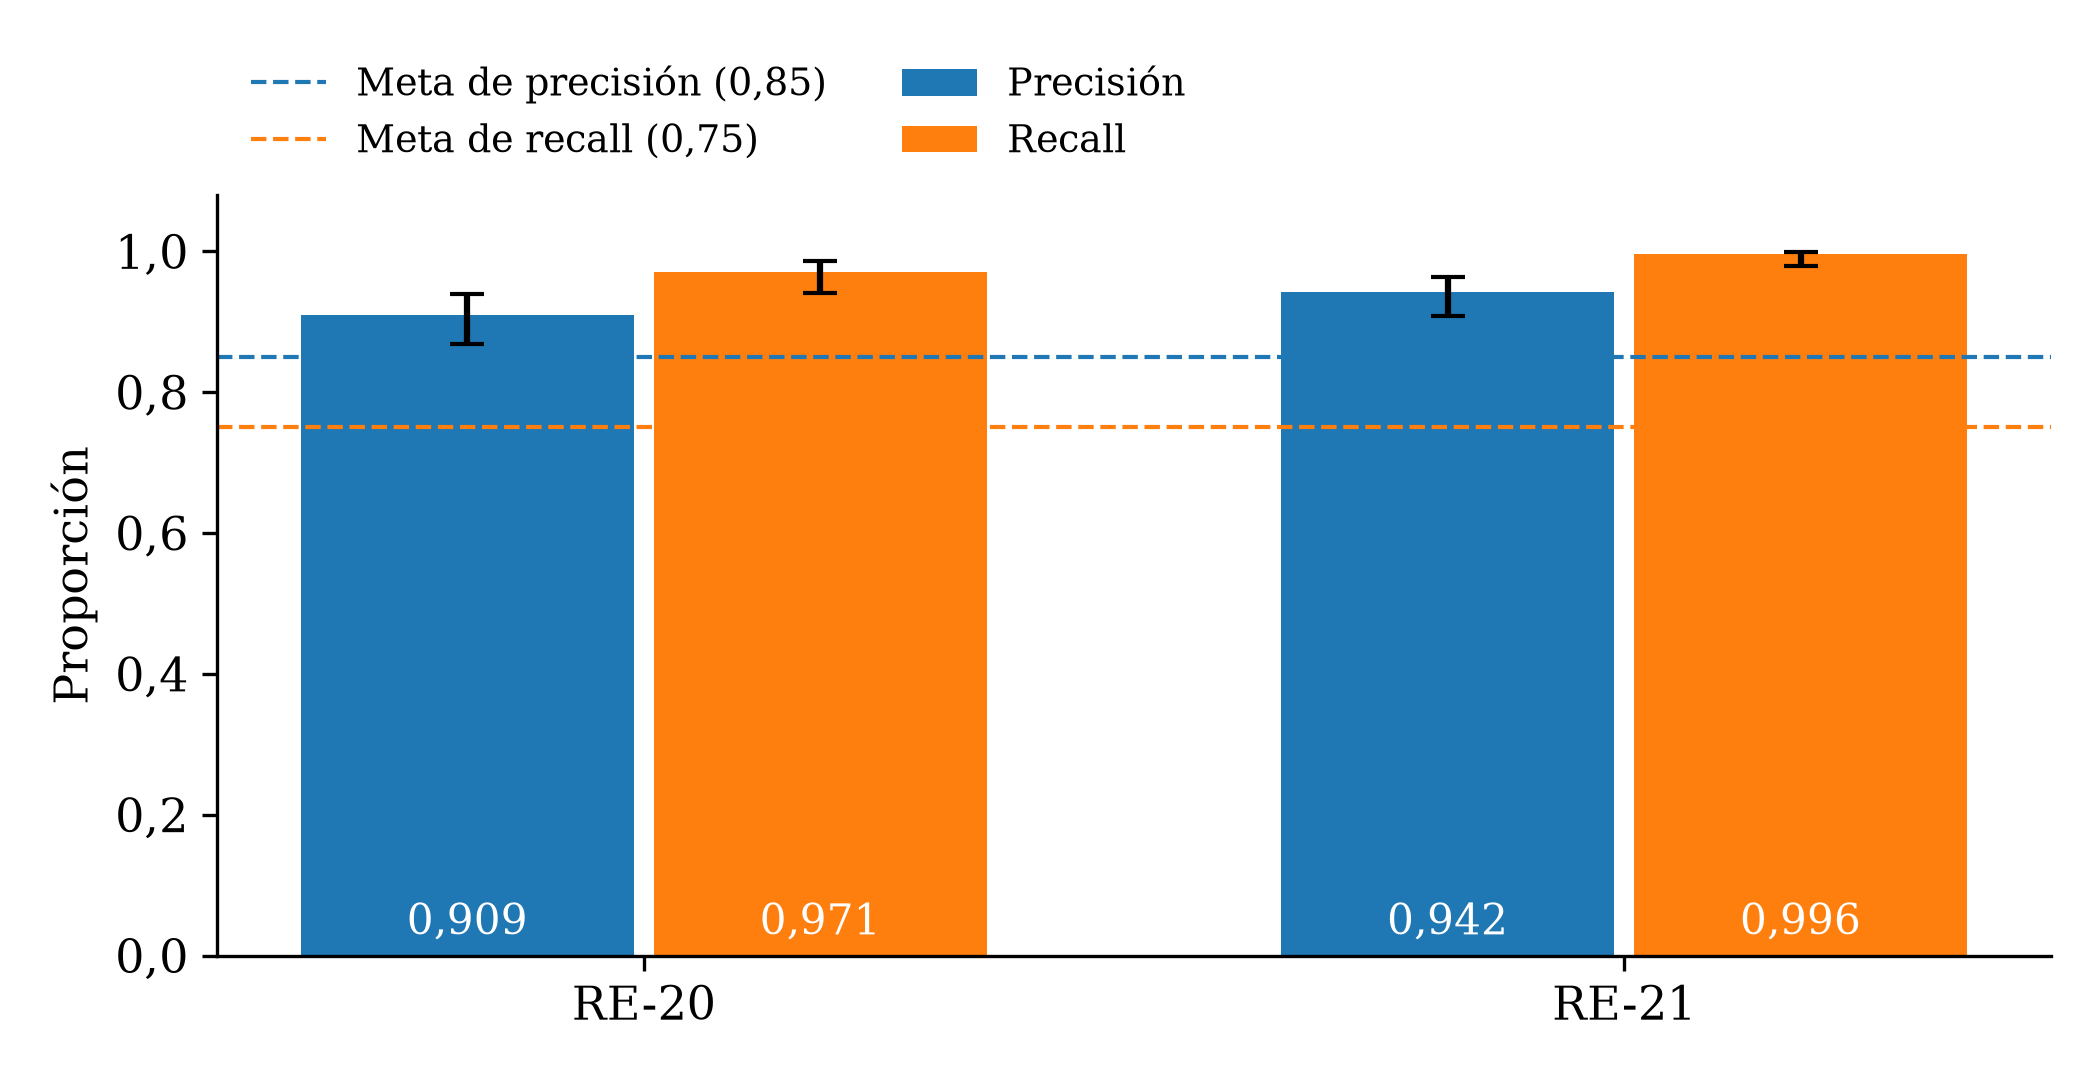
\includegraphics[width=\textwidth]{figuras/resultados/metricas-por-regla.png}
  \caption{Precisión y \emph{recall} por regla con su intervalo de confianza al 95 \% y las metas del producto}
  \label{fig:metricas-regla}
\end{figure}

\subsection{Aspectos de interpretación de los datos}

\subsubsection*{Qué significan los resultados}

El \emph{recall} alto indica que los evaluadores de RE-20 y RE-21 aplican bien los umbrales cuando reciben los datos correctos de la figura. La precisión depende de cuántas figuras rotadas tenga el conjunto. En este \emph{dataset} son 33 de 523, una proporción que fijó el diseño y que no se midió en manuscritos reales. Si en la revista las figuras rotadas fueran menos frecuentes, la precisión real sería mayor; si fueran más frecuentes, sería menor. Por eso la cifra global de precisión no debe leerse como una predicción del desempeño en producción. Lo que sí se puede afirmar es que el agente no produjo ningún falso positivo en las 463 figuras de píxeles que no estaban rotadas.

La precisión global también se beneficia de los documentos de Word. En ellos casi todas las figuras incumplen las reglas después de la conversión, de modo que reportar un incumplimiento casi siempre es correcto. El subconjunto de LaTeX es la medida más exigente, y en él la meta de precisión todavía no se cumple.

El tiempo medido corresponde a la extracción y al motor de reglas, ejecutados en un solo proceso y sin red. La redacción de sugerencias con Gemini todavía no está en el flujo y será la etapa más lenta. El requisito de tres minutos se debe volver a medir cuando esa etapa exista.

\subsubsection*{Relación con los antecedentes}

Esta evaluación usa documentos sintéticos con verdad de referencia conocida. Es el mismo camino que siguen, entre los antecedentes del Capítulo~\ref{cap:problematica}, los trabajos que generan documentos para no depender de anotaciones manuales \cite{ref18,ref22}. Los trabajos que verifican el formato de artículos \cite{ref5,ref9} reportan sus resultados sobre sus propios conjuntos de documentos y con reglas distintas, de modo que las cifras de esta tesis no son comparables de forma directa con las suyas.

\subsubsection*{Implicancias para la revista}

La regla RE-21 exige 300 dpi y el agente la verifica sobre el PDF. Los resultados muestran que un manuscrito preparado en Word no puede cumplirla, haga lo que haga el autor, porque la conversión reduce las imágenes. Si la revista recibe sobre todo manuscritos de Word, el agente observaría la resolución de casi todas las figuras y esas observaciones no le servirían al autor. Hay tres salidas posibles: pedir las figuras como archivos aparte, verificar la resolución sobre el documento de origen o ajustar el umbral para los PDF que provienen de Word. La decisión es editorial y se llevará a la revista. \pendiente{presentar este hallazgo al equipo editorial de Innosoft y registrar la decisión en \texttt{specs/00-producto.md}.}

\subsubsection*{Amenazas a la validez}

\begin{itemize}
  \item \textbf{Validez externa.} El \emph{dataset} es sintético. Mide si el agente detecta defectos controlados, no cómo se comporta con manuscritos reales, que tienen defectos que el generador no contempla: figuras compuestas por varias imágenes, capturas de pantalla, imágenes insertadas dentro de tablas. La evaluación con manuscritos reales y con editores está prevista en la Fase 2.
  \item \textbf{Circularidad.} El generador y el agente los escribió el mismo equipo. Esto se mitigó generando los PDF con LaTeX y Word, y no con la librería del agente, y verificando cada PDF con una segunda librería. La mitigación funcionó en parte: las tres causas de error encontradas son situaciones que el equipo no había previsto al escribir el agente.
  \item \textbf{Validez de constructo.} La verdad de referencia de las figuras recortadas se definió sobre la parte visible de la imagen. Las directrices de la revista no precisan este caso. Con la otra lectura posible, la de la imagen completa, los 5 falsos negativos de esa variante serían aciertos.
  \item \textbf{Cobertura.} Solo se evaluaron 2 reglas. El manifiesto ya registra defectos de pie de figura, numeración y mención en el texto en 47, 6 y 57 casos, que se evaluarán cuando esas reglas tengan evaluador.
  \item \textbf{Comparaciones múltiples.} Se hicieron varias pruebas de hipótesis sin corregir el nivel de significancia. Los valores p de las conclusiones principales son lo bastante pequeños como para que una corrección no las cambie, salvo la diferencia entre generadores en RE-21 ($p = 0{,}016$), que debe tomarse con cautela.
  \item \textbf{Entorno.} Los tiempos se midieron en un equipo de desarrollo con Windows 11 y dependen de él.
\end{itemize}

\subsubsection*{Reproducibilidad}

El generador, el evaluador y los resultados están en el repositorio, en \texttt{agente/\allowbreak{}tools/\allowbreak{}eval\_dataset/} y \texttt{agente/\allowbreak{}evaluacion/}. La misma semilla produce el mismo plan de documentos y la misma verdad de referencia. Los PDF no se versionan porque se regeneran con un solo comando.
